\section{Kinematics}

\begin{defn}{Displacement $s$}{}
Distance moved in a specific direction. 
\end{defn} 
Graphically, change in displacement is the area under a velocity-time graph.

\begin{defn}{Velocity $v$}{}
Rate of change of displacement with respect to time. 
\begin{equation} 
v = \odv{s}{t} 
\end{equation}
\end{defn} 
Graphically, velocity is the gradient of a displacement-time graph; change in displacement is the area under a velocity-time graph.

\begin{defn}{Acceleration $a$}{}
Rate of change of velocity with respect to time. 
\begin{equation} 
a = \odv{v}{t}
\end{equation}
\end{defn} 
Graphically, acceleration is the gradient of a velocity-time graph; change in velocity is the area under an acceleration-time graph.

\subsection{Rectilinear motion}
The following \textbf{equations of motion} only hold for \underline{uniformly accelerated} motion in a \underline{straight line}.

\begin{equation}\label{eqn_mtn1} v=u+at \end{equation}

\begin{equation}\label{eqn_mtn2} s=\frac{1}{2}(u+v)t \end{equation}

\begin{equation}\label{eqn_mtn3} s=ut+\frac{1}{2}at^2 \end{equation}

\begin{equation}\label{eqn_mtn4} v^2=u^2+2as \end{equation}

\deriv{See Appendix for the derivation.}

\subsection{Projectile motion}
\begin{defn}{Projectile motion}{}
Motion due to
\begin{itemize}
\item \textbf{uniform velocity} in one direction, and
\item \textbf{uniform acceleration} in a perpendicular direction.
\end{itemize}
\end{defn}

Analyse horizontal motion in the $x$-direction, and vertical motion in the $y$-direction separately. Resolving velocity into components,
\[ v_x = v \cos \theta, \tab v_y = v \sin \theta \]
\[ v = \sqrt{{v_x}^2+{v_y}^2} \tab \theta = \tan^{-1} \frac{v_y}{v_x} \]

\subsubsection{Horizontal motion}
Horizontal motion does not undergo acceleration; hence, horizontal velocity remains constant.
\[ v_x = u_x \]
\[ s_x = v_x t \]

\subsubsection{Vertical motion}
Vertical motion undergoes acceleration due to gravity $g$; hence, vertical velocity changes.
\[ v_y = u_y - gt \]
\[ s_y = \frac{1}{2} (u_y + v_y) t \]
\[ s_y = u_y t - \frac{1}{2} g t^2 \]
\[ {v_y}^2 = {u_y}^2 - 2gs_y \]

\subsubsection{Relevant quantities}
The following quantities should be derived and not memorised.

\textbf{Time of flight}:
\begin{align*}
v_y &= u_y - gt \\
0 &= u \sin \theta  - gt \\
t &= \frac{u \sin \theta}{g}
\end{align*}
\[ \boxed{t_{\text{flight}} = \frac{2u \sin \theta}{g}} \]

\textbf{Maximum height}:
\begin{align*}
{v_y}^2 &= {u_y}^2 - 2gs_y \\
0 &= (u \sin \theta)^2 - 2gh
\end{align*}
\[ \boxed{h = \frac{u^2 \sin^2 \theta}{2g}} \]

\textbf{Range}:
\begin{align*}
R &= u_x t_{\text{flight}} \\
R &= u \cos \theta \cdot \frac{2u \sin \theta}{g}
\end{align*}
\[ \boxed{R = \frac{u^2 \sin 2\theta}{g}} \]
Range is maximum when $\theta = 45\degree$, then maximum range $R = \dfrac{u^2}{g}$.
\pagebreak

\subsubsection{Effect of air resistance}
\begin{table}[H]
\centering
\begin{tabular}{p{0.5\textwidth}p{0.5\textwidth}}
\hline\hline
Air resistance is negligible & Air resistance is not negligible \\
\hline
\begin{itemize}
\item Horizontal velocity: remains unchanged

No horizontal deceleration.

\item Vertical velocity: increases from zero with constant rate downward at the acceleration of free fall

Resultant force on the stone is only its weight alone, which is constant, hence constant vertical deceleration.
\end{itemize} & 
\begin{itemize}
\item Horizontal velocity: decreases at a decreasing rate

Air resistance becomes smaller with time due to diminishing horizontal velocity; horizontal velocity asymptotically approaches zero.

\item Vertical velocity: increases from zero at a decreasing rate

Acceleration decreases due to reduction of resultant downward force (air resistance opposing motion increases as speed increases).

\item Time of flight for downward motion is longer than upward motion, because net downward acceleration (weight - air resistance) is smaller than net upward deceleration (weight + air resistance).
\end{itemize} \\
\hline\hline
\end{tabular}
\end{table}

Characteristics of path of object with non-negligible air resistance:
\begin{enumerate}
    \item Lower maximum height, displaced to the left
    \item Asymmetrical shape
    \item Shorter range
\end{enumerate}

\begin{figure}[H]
\centering
\begin{tikzpicture}
  \begin{axis}%
    [axis lines=middle,
     enlargelimits={abs=0.2},
     xlabel = $x$,
     ylabel = $y$,
     ticks=none
    ]
    \addplot[domain=0:10,samples=200,smooth,red] {-(x-5)^2 + 25};
    \addplot[domain=0:4,samples=200,smooth,blue] {-(x-4)^2 + 16};
    \addplot[domain=4:6.52,samples=200,smooth,blue] {-(x-4)^3 + 16};
  \end{axis}
\end{tikzpicture}
\end{figure}
\pagebreak

\subsection{Problems}
\begin{prbm}
A tree is wet after a rain and slowly drips water, with one droplet falling from rest every $t = 1$ \unit{s}. At any time, exactly $n = 5$ droplets can be observed mid-air. Determine the height $h$ of the tree. Neglect air resistance.

\textit{Leave your answer to $2$ significant figures in units of \unit{m}}.

\begin{figure}[H]
    \centering
    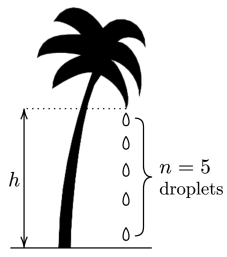
\includegraphics{images/Wet_Tree.png}
\end{figure}
\end{prbm}

\begin{proof}[Solution]
Consider the falling motion of a single droplet. Let the time taken for the droplet to reach the ground be $T$. From kinematics, we have:
\[ h = \frac{1}{2} gT^2 \]
Throughout the duration of its fall, an additional $n$ droplets must have fallen from the tree, such that the $n$-th additional droplet falls exactly when the initial droplet hits the ground. This condition is necessary to ensure that there are always $n$ droplets falling mid-air. Hence, $T$ must be related to $t$ by:
\[ T = nt \]
We can then solve for $h$:
\begin{align*}
h &= \frac{1}{2}g(nt)^2 \\
\Aboxed{h &\approx 120\:\unit{m}}
\end{align*}
\end{proof}
\pagebreak

\begin{prbm}[The Monkey and the Hunter Problem]
A student fires a dart at a stuff monkey held by an electromagnet a distance $h$ vertically above the dart gun and a distance $R$ horizontally away from the dart gun. The student aims directly at the monkey and fires, but as the student fires, the power of the electromagnet is turned off, causing the monkey to drop simultaneously. Will the dart hit the monkey?
\end{prbm}

\begin{figure}[H]
    \centering
    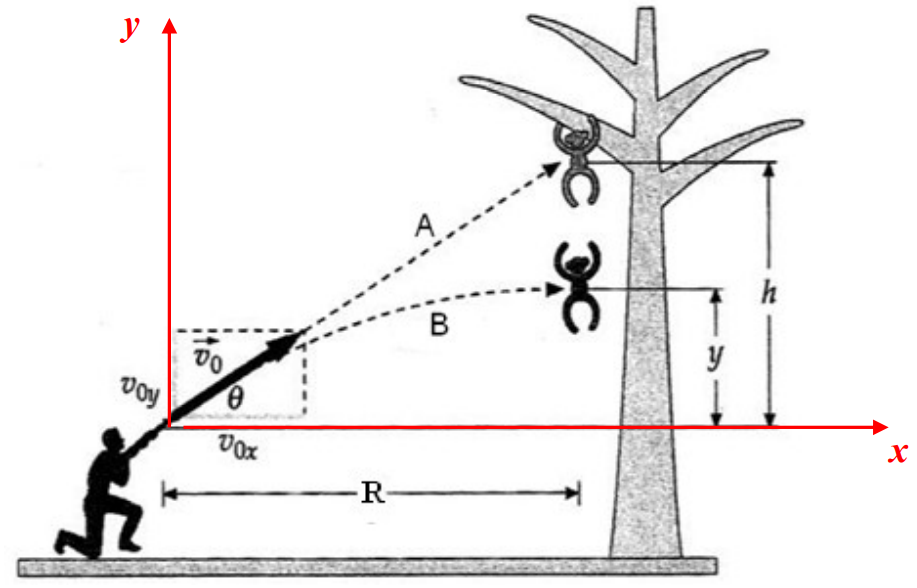
\includegraphics[width=12cm]{images/Monkey_hunter.png}
\end{figure}

\begin{solution}
It takes time $t$ the dart to travel a horizontal distance $R$:
\[ t=\frac{R}{v_0\cos\theta} \]

At time $t$,
\[ y_d=v_0\sin\theta t-\frac{1}{2}gt^2,\:y_m=h-\frac{1}{2}gt^2 \]

Difference in $y$-position at time $t$:
\begin{align*}
y_d-y_m 
&= \brac{v_0\sin\theta t - \frac{1}{2}gt^2} - \brac{h-\frac{1}{2}gt^2} \\
&= v_0\sin\theta t - h \\
&= v_0\sin\theta\frac{R}{v_0\cos\theta}-h \\
&= R\tan\theta - h \\
&= R\brac{\frac{h}{R}}-h = 0
\end{align*}
Therefore, the dart will hit the monkey.
\end{solution}
\pagebreak

\begin{prbm}
As the ball here rolls down the hill as shown in the figure below, describe the variation in its speed and acceleration.
\begin{figure}[H]
    \centering
    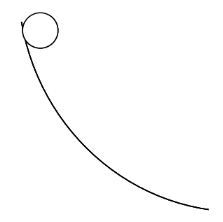
\includegraphics[width=5cm]{images/ball_roll.png}
\end{figure}
\end{prbm}

\begin{proof}[Answer]
Slope of the hill gets gentler as the ball rolls down, so \textbf{acceleration decreases}. 

Though acceleration decreases, it is always acting downwards, so \textbf{speed increases} due to the conversion of gravitational potential energy to kinetic energy (conservation of energy).
\end{proof}

\pagebreak